\chapter[Literature Review]{Literature}

\section{Domain-Specific Languages (DSLs)}
Declarative domain-specific languages (DSLs) have made a big impact on compiler optimization by offering targeted solutions for specific optimization tasks. For example, Halide \cite{Jonathan2018} is a domain-specific language and compiler framework designed to optimize image processing and computational photography. Writing efficient code for image processing often requires complex optimizations to exploit parallelism and memory locality. In Halide, the algorithm specifies the computational logic for these tasks, detailing what needs to be done, such as resizing, sharpening, or blurring an image. The schedule defines the execution strategy, including how computations are ordered, parallelized, and managed in memory. This separation of concerns allows Halide to generate highly optimized code by focusing on both the functional description and the efficient execution of tasks. Elevate \cite{Hagedorn2020} is another functional language designed to let programmers define custom optimization strategies. It allows for creating composable optimizations rather than sticking to predefined APIs. Its success in case studies and practical applications highlights its ability to handle complex optimization tasks and deliver strong performance.

\begin{figure}[h]
    \centering
    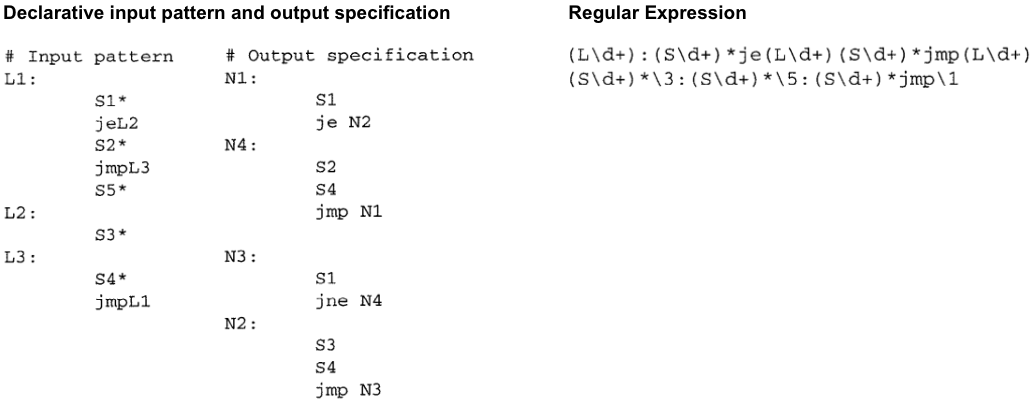
\includegraphics[width=1\textwidth]{Packages/regex.png}
    \caption{Example of Optimizer Patterns and Regular Expression \cite{Spinellis1999}}
    \label{figure:regex}
\end{figure}

Spinellis created a peephole optimizer that uses a declarative DSL to specify optimizations \cite{Spinellis1999}. Spinellis transformed specifications into string regular expressions, which are then applied to the target code, allowing for adaptive and efficient refinements. \autoref{figure:regex} illustrates an example of this framework. On the left of the figure is a declarative specification for the one-bit loop optimization \cite{Spinellis1999}. The input pattern is parsed and translated into the regular expression in the right part of the figure. The optimizer uses regular expressions to find matches in the program and transform and optimize the code iteratively.

\section{Logic Programming Languages}
DataLog has established itself as a powerful tool in compiler implementation through its applications in complex program analysis and transformation. 
For instance, the Soufflé Datalog engine \cite{silverman2021wantanalyzeschemeprograms} introduces a new method for control-flow analysis in Scheme, making it possible to perform scalable and complex analyses of functional programming constructs, and extending the benefits of Datalog-based static analysis to Scheme-like languages. Similarly, DIMPLE \cite{Benton2007}, a framework for Java bytecode static analyses, is implemented in the Yap Prolog system. DIMPLE leverages logic programming capabilities to provide a declarative language for specifying analyses and representing Java bytecodes. The framework facilitates iterative experimentation and delivers efficient implementations that are on par with specialized tools. 

Another example is the Doop framework \cite{Bravenboer2009} which utilizes Datalog to offer a declarative solution for points-to analysis in Java, providing impressive performance gains and scalability for precise context-sensitive analyses. \autoref{figure:doop} illustrates a Datadog rule that Doop uses to represent a call graph. The query finds and returns a call graph edge if all of the predicates inside \texttt{CallGraphEdge} are true. First, it queries the properties of the virtual method call \texttt{call} including its receive object \texttt{base}, \texttt{name}, and \texttt{descriptor}. After that, it queries the \texttt{heap} that this \texttt{base} object is pointing to and checks for the type of that \texttt{heap} object. Finally, it queries method lookups for the method that is being called from the \texttt{heaptype}.

\begin{figure}[h]
    \centering
    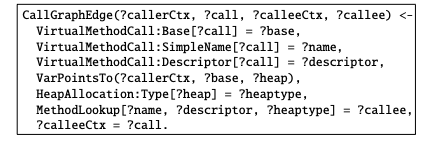
\includegraphics[width=0.6\textwidth]{Packages/Doop.png}
    \caption{DOOP's rule for virtual method invocations \cite{Bravenboer2009}}
    \label{figure:doop}
\end{figure}

Lam et al. developed a framework using Datalog queries and a specialized language called PQL, which employs deductive databases and binary decision diagrams (BDDs) to tackle complex issues like pointer aliasing and heap object management in a context-sensitive manner \cite{Lam2005}. PQL helps simplify the process by allowing programmers to write queries in a more intuitive way. Instead of needing to understand the underlying database details, programmers can write code patterns in Java that are automatically converted into Datalog. \autoref{figure:pql} provides an example of a query for simple SQL injection written in PQL and the equivalent Datadog rules. The SQL injection can be caught by checking if the parameter returned from calling \texttt{getParameter} on a \texttt{HttpServletRequest} is then passed directly as an argument to an \texttt{execution} call on the database \texttt{Connection}. Similarly, Datadog rules first check if there exists a method call to \texttt{getParameter} with a return value stored in a \texttt{v1} variable pointing to a heap object \texttt{h}. After that, it checks if there exists an invocation of \texttt{execute} with an argument \texttt{v2} also pointing to the object \texttt{h}.

\begin{figure}[h]
    \centering
    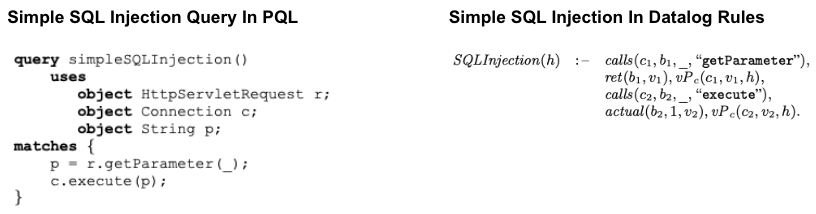
\includegraphics[width=1\textwidth]{Packages/PQL.png}
    \caption{Simple SQL Injection Example in PQL \cite{Lam2005}}
    \label{figure:pql}
\end{figure}

\newpage
\section{Transformation, Rewriting Techniques, and Verification}
Transformation and rewriting techniques are essential to modern compiler optimization, enabling sophisticated processes like grammar specification, pattern matching, and program rewriting. Stratego~\cite{Eelco2001} is a language designed for specifying program transformation systems using rewriting strategies, which allow for precise control over rule application. The compiler transforms these rules into C code and leverages the ATerm library for effective term representation. It has been used in several applications, including program transformation tools like XT, and domain-specific optimization frameworks like CodeBoost ~\cite{Eelco2001}. On the other hand, Veriopt \cite{Webb2023} offers a comprehensive framework for formal verification of Graal compiler optimizations. This framework employs  ``term rewriting rules on the abstract term representation" \cite{Webb2023} and then maps these rules to term graph transformations. In the Veriopt project, a term rewriting system, also known as an optimization phase, comprises a set of rules that can be applied repeatedly to optimize expressions. Each phase is associated with different types of root nodes in patterns, such as AddNode, AbsNode, and MulNode. 

\begin{figure}[h]
    \centering
    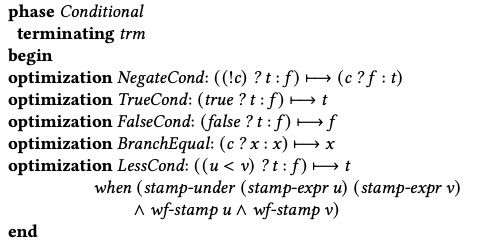
\includegraphics[width=0.6\textwidth]{Packages/veriopt.png}
    \caption{Conditional canonicalization rules \cite{Webb2023}}
    \label{figure:veriopt}
\end{figure}

\autoref{figure:veriopt} provides an example of such an optimization phase tailored for conditional expressions. NegateCond transforms negated conditions using logical equivalences, while TrueCond simplifies expressions where the condition is always true by directly applying the true outcome. Conversely, FalseCond addresses conditions that are always false by eliminating irrelevant branches. BranchEqual simplifies expressions with equality checks by optimizing or removing redundant comparisons.

\section{Identified Research Gaps}
Despite the established effectiveness of logic programming languages like Datalog in program analysis, there is limited research on integrating these techniques within modern compiler frameworks such as GraalVM. While significant advancements have been made in transformation and rewriting techniques using domain-specific languages (DSLs) and other paradigms, there is a notable absence of comparative studies on incorporating logic programming-based optimizations into GraalVM. This gap extends to a lack of empirical evidence assessing the impact of such techniques on optimization time and efficiency. Integrating Prolog-based rules with GraalVM’s graph-based IR is particularly challenging due to insufficient research on mapping Graal IR to Prolog and ensuring that Prolog-based optimizers work effectively within the Java environment. Addressing these challenges could enhance our understanding of how to apply logic programming in modern compilers and improve compiler optimization practices by providing valuable insights into the performance and effectiveness of these techniques.
